\subsection{Worksheet - Intro to Coupled Oscillators}
\begin{p}
Give some examples of coupled oscillators.
\end{p}
\begin{s}
\phantom{i}
\begin{itemize}
    \item Masses coupled together by springs
    \item A crystal lattice, which can be approximated as atoms being connected by springs in a lattice structure
    \item Molecules (e.g. CO2) which we can treat as a carbon atom connected linearly to two oxygen atoms.
\end{itemize}
\end{s}

\begin{center}
    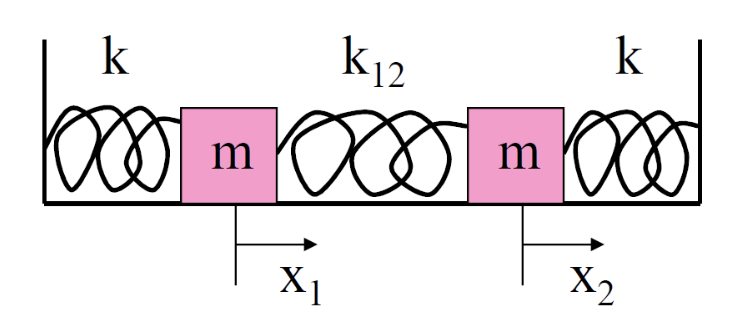
\includegraphics[scale=0.5]{Lecture-10/w10-img1.png}
\end{center}
\begin{p}
Find the Lagrangian for the two coupled oscillators(two masses connected by springs). Find the equations of motion.
\end{p}
\begin{s}
The Lagrangian is given by:
\[\LL = T - U = \frac{m}{2}\left(\dot{x}^2_1 + \dot{x}^2_2\right) - \left[\frac{k}{2}x_1^2 + \frac{k_{12}}{2}(x_1 - x_2)^2 + \frac{k}{2}x_2^2\right]\]
To obtain the equations of motion, we use the EL equations:
\[\dod{}{t}\dpd{\LL}{\dot{x}_1} = m\ddot{x}_1 = \dpd{\LL}{x_1} = -kx_1 - k_{12}x_1 + k_{12}x_2\]
\[\dod{}{t}\dpd{\LL}{\dot{x}_2} = m\ddot{x}_2 = \dpd{\LL}{x_2} = -kx_2 - k_{12}x_2 + k_{12}x_1\]
Which agrees with our analysis using the Newtonian formulation. This is clearly a coupled system of ODEs. To start solving this, we start by writing this in a nicer form, defining a column vector $\v{x} = \m{x_1 \\ x_2}$. This transforms things into a matrix equation:
$$\left(\begin{array}{cc}m & 0 \\ 0 & m\end{array}\right)\left(\begin{array}{c}\ddot{x}_{1} \\ \ddot{x}_{2}\end{array}\right)=-\left(\begin{array}{cc}k+k_{12} & -k_{12} \\ -k_{12} & k+k_{12}\end{array}\right)\left(\begin{array}{c}x_{1} \\ x_{2}\end{array}\right)$$
Which we can write as:
\[\MM\ddot{\v{x}} = -\KK\v{x}\]
\end{s}

\begin{p}
Using the complex quantity $\v{z} = \v{a}\exp(i\omega t)$, show that the equation for the normal modes can be written as $(\KK - \omega^2\MM)\v{a} = 0$.
\end{p}
\begin{s}
We define the complex quantity $\v{z}$ as above (such that $\v{x} = \Re\v{z}$, and then we have:
\[\MM\ddot{\v{z}} = \MM\v{a}(-\omega^2)\exp(i\omega t) = -\KK\v{a}\exp(i\omega t)\]
Then cancelling out the exponentials, we have:
\[\KK\v{a} = \MM\omega^2\v{a}\]
Rearranging, we have:
\[(\KK - \omega^2\MM)\v{a} = 0\]
This is an \textbf{eigenvalue problem}, which we are familiar with from linear algebra. We note that here, $\MM$ is just an identity matrix multiplied by $m$.
\end{s}

\begin{p}
Write out the characteristic equation. What are the roots? (i.e. the eigenfrequencies).
\end{p}
\begin{s}
To solve this eigenvalue problem (i.e. for the system to have nontrivial solutions) we require that $\det(\KK - \omega^2\MM) = 0$. This is a polynomial/characteristic equation, for which the solution are the eigenvalues. For $\MM$, $\KK$ as we have defined them, this looks like:
\[\det(\KK - \omega^2\MM) = (k + k_{12}- m\omega^2)^2 - k_{12}^2 = 0\]
Where the first term is the product of the diagonals and the second term is the product of the off diagonals. Factoring, we have:
\[(k - m\omega^2)(k + 2_{k12} - m\omega^2) = 0\]
So the characterstic equation hence has the two roots of:
\[\omega_1 = \sqrt{\frac{k + 2k_{12}}{m}}, \omega_2 = \sqrt{\frac{k}{m}}\]
The types of motion described by these two eigenfrequencies are as follows. For $\omega_1$, the blocks move with the same frequency and exactly out of phase. For $\omega_2$, the blocks move with the same frequency, and exactly in phase. We will see why this is in the last two question, by solving for the amplitudes $a_1, a_2$.
\end{s}

\begin{p}
Find the normal mode corresponding to the eigenfrequency $\sqrt{k/m}$.
\end{p}
\begin{s}
To find the normal mode, we solve for the eigenvector corresponding to the above eigenfrequency/eigenvalue:
\[(\KK - \omega_2\MM)\m{a_1 \\ a_2} = \m{k_{12} & - k_{12} \\ -k_{12} & k_{12}}\m{a_1 \\ a_2} = 0\]
Or equivalently:
\[k_{12}\m{1 & -1 \\ -1 & 1}\m{a_1 \\ a_2} = 0\]
From which we can see that the restriction on $a_1, a_2$ (remeber that they are complex) is that:
\[a_1 = a_2 = A\exp(-i\delta)\]
Hence solving for $\v{z}$:
\[\v{z} = \m{a_1 \\ a_2}\exp(i\omega_2 t) = \m{A \\ A}\exp(i(\omega_2 t - \delta))\]
Therefore, finding $\v{x}$ we have:
\[\v{x}_{II} = \Re\v{z} = \m{A \\ A}\cos(\omega_2 t - \delta)\]
This is an eigenmode, at the lower frequency. We can see from this that the two masses oscillate in phase with each other.
\end{s}

\begin{p}
Find the normal mode corresponding to the eigenfrequency $\sqrt{(k+2k_{12})/m}$.
\end{p}
\begin{s}
Similarly solving for the eigenvector, we have:
\[(\KK - \omega^2\MM)\v{a} = \m{-k_{12} & -k_{12} \\ -k_{12} & -k_{12}}\v{a} = -k_{12}\m{1 & 1 \\ 1 & 1}\m{a_1 \\ a_2} = 0\]
Therefore we obtain the requirement that $a_1 = -a_2$, and hence:
\[\v{x}_I = \m{A \\ -A}\cos(\omega_1 t - \delta)\]
\end{s}

\begin{p}
What is the general solution?
\end{p}
\begin{s}
The general solution is the sum of the eigenmodes:
\[\v{x}(t) = \v{x}_I(t) + \v{x}_{II}(t)\]
\end{s}

\begin{p}
If block 1 oscillates while block 2 is held fixed, what is the frequency of oscillations?
\end{p}
\begin{s}
The frequency of oscillations of the first block would be given by $\omega_0 = \sqrt{\frac{k + k_{12}}{m}}$; the reasoning for this is the block feels a restoring force $-kx$ from the left, restoring force $k_{12}x$ from the right, which leads to an effective spring constant $k + k_{12}$ and hence leads to the solution as stated.
\end{s}

\begin{p}
How does the uncoupled frequency above compare to the two eigenfrequencies?
\end{p}
\begin{s}
\[\omega_2 < \omega_0 < \omega_1\]
\end{s}
\noindent$\omega_2$ is the frequency of the lowest mode, the blocks are in phase. The middle frequency is where we fix one block and just let the other oscillate. $\omega_1$ corresponds to the higher eigenmode, with the blocks oscillating out of phase, at the highest frequency. Next day, we will look at coupled pendulums and normal coordinates (which is changing bases to diagonalize our matrices), where we obtain the useful result that the normal coordinates are independent of one another.

\begin{p}
If the coupling is weak ($k_{12} \ll k$), what is an approximate expression for the frequency $\omega_0=\sqrt{\frac{k+k_{12}}{m}}$?
\end{p}
\begin{s}
We apply Taylor expansion:

\[ \omega_0=\sqrt{\frac{k}{m}\left(1+\frac{k_{12}}{k}\right)}\approx\sqrt{\frac{k}{m}}\left( 1+\frac{k_{12}}{2k} \right) \]
\end{s}